\documentclass{article}
\title{Political Information in Bureaucratic Policymaking}
\author{Devin Judge-Lord} % \\ JudgeLord@Wisc.edu}
\date{\today} 

\date{\today} 
 %\setlength{\parskip}{1em}
% \usepackage[round, sort, comma]{natbib}
% \setcitestyle{notesep={, },round,aysep={},yysep={,}}

%\setlength{\parindent}{0pt}

% \usepackage[authordate,strict,backend=bibtex8,babel=other, doi=false, url=false, isbn=false, uniquename=false, maxcitenames = 2, uniquelist=false,%
% bibencoding=inputenc, natbib]{biblatex-chicago}
%\usepackage[authordate, backend=biber, doi=false, url=false, isbn=false, uniquename=false, maxcitenames = 2, uniquelist=false, natbib]{biblatex-chicago}



% ---------------------------------------
%   REFERENCES
% ---------------------------------------
\usepackage{natbib} %[round, sort, comma]{natbib}
  \bibpunct[: ]{(}{)}{;}{a}{}{,}
%\usepackage[nottoc,numbib]{tocbibind} % numbers bib. in table of contents


% ---------------------------------------
%   MARGINS AND SPACING
% ---------------------------------------
\usepackage[margin=1in]{geometry} 
\usepackage{setspace} % line spacing


% ---------------------------------------
%   TABLES AND FIGURES
% ---------------------------------------
\usepackage{graphicx} % input graphics
\graphicspath{ {./Figs/} }

\usepackage{float} % float parameters
\usepackage{placeins} % \FloatBarrier: prevent floats spilling across sections
\usepackage{subcaption} % subfloats with individual captions
\usepackage{multirow} % multicolumn and multirow
\usepackage{booktabs} %? for toprule, midrule etc
\usepackage{dcolumn} % decimal-aligned columns

\usepackage{tikz}
\usetikzlibrary{positioning}
\usetikzlibrary{shapes.geometric}
\usetikzlibrary[patterns]

% ---------------------------------------
%   MATH
% ---------------------------------------
\usepackage{amsmath}
%  Math symbols (depends on whether you customize typeface)
%  \usepackage{amsfonts}
%  \usepackage{mathrsfs}
\usepackage{amssymb}
  %  \newcommand{\E}{\mathrm{E}}
  %  \newcommand{\Var}{\mathrm{Var}}
  %  \newcommand{\Cov}{\mathrm{Cov}}
  %  \newcommand{\plim}{\mathrm{plim}}
  %  \renewcommand{\L}{\mathcal{L}}
  %  \renewcommand{\d}{\mathrm{d}}
  %  \newcommand{\R}{\mathbb{R}}


% ---------------------------------------
%   TYPEFACE AND TEXT STYLES
% ---------------------------------------


% \usepackage{fontenc} 
% advisable to include for nitty-gritty details
% (ligatures, kerning & other typographical things)

% \usepackage[usenames, dvipsnames]{xcolor} % extra colors
\usepackage{hyperref} % hyperlinks
   \hypersetup{
     colorlinks = true, 
     citecolor = black, 
     linkcolor = blue,
     urlcolor = blue}

\usepackage{comment} % provides {comment} environment
\usepackage{enumitem} % allows [nosep] option for lists

\usepackage{endnotes}

\makeatletter
\renewcommand\@makeenmark{%
  \textsuperscript{\normalfont\textcolor{blue}{\@theenmark}}%
}
\newcommand{\uncolormarkers}{%
  \renewcommand\@makeenmark{%
    \textsuperscript{\normalfont\@theenmark}%
  }%
}
\makeatother


\newcommand{\exclude}[1]{\StopSearching ##1\StartSearching}

\usepackage{ragged2e}

\let\footnote=\endnote
\begin{document}

\maketitle
%  \tableofcontents
% \abstract{This dissertation is about public pressure campaigns that target U.S. federal agency rulemaking, a technocratic policy process in which participation is usually limited to a few policy insiders. Occasionally, however, public pressure campaigns help make agency rules some of the most hotly contested policies of our time. I examine who organizes public pressure campaigns and why, whether these campaigns affect congressional oversight, and whether they affect policy. Answering these questions informs our understanding of bureaucratic politics as well as interest group lobbying, organizing, and mobilizing tactics. Most comments that federal agencies receive on their draft policies come from ordinary people who were inspired by a public pressure campaign. Yet leading theories of bureaucratic policymaking neither explain nor account for these occasional bursts of civic engagement. This dissertation develops and tests theories about the roles of individuals, organizations, coalitions, and social movements in bureaucratic policymaking. I argue that pressure campaigns build movements, attract policymakers' attention, and systematically counter corporate power by generating political information---information about public demands.   I make four main contributions:
  
  First, drawing on scholarship on social movements, interest group behavior, and lobbying, I identify three reasons for lobbying organizations to mobilize ordinary people. Each logic suggests a different observable pattern of public engagement, and I analyze millions of public comments on thousands of agency rules to develop the first systematic measures of public engagement in bureaucratic policymaking. Contrary to other forms of lobbying, I find that mass comment campaigns are almost always a conflict expansion tactic rather than well-resourced groups creating an impression of public support. Most public comments are mobilized by public interest organizations, not by narrow private interests or astroturf campaigns. However, the resources and capacities required to launch a campaign cause a few larger policy advocacy organizations to dominate.
  
  Second, building on theories of political oversight, I theorize that mass engagement in bureaucratic policymaking may alert elected officials to political opportunities and risks, thus affecting oversight behavior. I assess this argument by analyzing correspondence between members of Congress and agency officials on proposed rules with and without mass engagement. I find that public pressure campaigns are correlated with congressional attention and that coalitions with more congressional support are more likely to achieve their policy goals.
  
  Third, I integrate intuitions about outside lobbying and oversight into a broader theory of how public pressure campaigns may affect policy by producing potentially influential political information. I suggest four causal mechanisms by which lobbying may influence bureaucrats and expand leading formal models of interest group influence in bureaucratic policymaking to account for political information. I then test these models using a mix of hand-coding and computational text analysis methods.   
  
  Fourth, I advance the literature on social movement pressure through a case study of the environmental justice movement. I show that pressure campaigns are more than a lobbying tactic; they are also an institutionalized form of contentious politics over the distribution of governmental power. I examine the discursive effects of environmental justice claims both qualitatively and quantitatively, including the role of Native activists and environmental groups in shaping federal policy. I find that agencies frequently ignore environmental justice concerns but are more likely to add language addressing environmental justice in their final rules when public comments raise environmental justice concerns. I conclude with implications for theories of bureaucratic policymaking and future research, a review of dominant ways of thinking about public comment periods, and proposed reforms for public participation in policymaking.}
% \newpage
%  \onehalfspace

This dissertation is about ordinary peoples' input on policies made by bureaucrats. People may believe that their voices matter, but it is unclear if they do or ought to. I analyze millions of public comments on thousands of agency rules to develop the first systematic measures of mass engagement in bureaucratic policymaking. I theorize that mass engagement may, in limited circumstances, influence bureaucrats by shifting their incentives or evoking powerful norms. Using my new measures to assess these mechanisms, I show how various parts of the U.S. government respond to ordinary peoples' input.  %aims to understand the effects of public attention on executive-branch policymaking.

Democracies face two big problems. First, they are vulnerable to fleeting passions and demagogues. To combat this, they leave many decisions to experts who, ideally, use wisdom and judgment loosely guided by the public. Second, everyone cannot vote on every decision. Thus, they delegate power to representatives (who then delegate it to deputies), create temporary mini-publics\footnote{
As imagined by \citet{Dahl1989}, mini-publics are representative, selected at random, and deliberative. Besides juries, however, deliberative and randomly-selected bodies are rare. Instead, citizens more often engage in government decisions where they opt-in, such as hearings, petitions, and public comment periods. These mechanisms of public input generate a different, more contentious flavor of public input.
}, 
and solicit input from those most affected or moved by a public decision. Most policy is then made by bureaucrats\footnote{
By one estimate upward of 90\% of legally binding U.S. federal policy is now written by agencies \citep{West2013}.
}, supposedly guided indirectly through elected representatives and directly by limited public input\footnote{
Agencies advertise public comment periods as an opportunity for a voice in government decisions. Commenting on proposed agency rules is described as ``an important part of democracy'' (WSJ 2017), the ``purest example of participatory democracy in actual American governance'' \citep{Herz2016}. \citet{Rossi1997} finds that ``courts, Congress, and scholars have elevated participation [in rulemaking] to a sacrosanct status...greater participation is generally viewed as contributing to the democracy.'' % Is it?
% Both of these problems converge in the bureaucracy, run by experts who are deputized by elected officials (or by their deputy's deputy's deputy) and with procedures that create opportunities for public input. It is far from clear how bureaucratic decisions are to balance expertise, accountability to elected officials, and responsiveness to public input in decisionmaking. 

% \paragraph{The politics of agency decisions:} 
Expertise, delegation, and limited public input thus converge in bureaucratic policymaking, where bureaucrats are required to use reasoned judgment, be accountable to elected officials, and be responsive to public input. There is no normative consensus on how to rank or merge these aims.
Administrative procedures for gathering input and their justifications cite all three.
}, 
but may still be contentious.
% This process may be contentious.
% Occasionally, this is contentious.
% These solutions raise new problems.
% This is the subject of my study.
% We still have much to learn 

Leading models of bureaucratic policymaking focus either on how agencies learn about policy problems and solutions, negotiate or avoid accountability to various elected officials, or balance interest-group demands.\footnote{
On learning, see \citet{Libgober2018} for an information-based model where commenting reveals information to the agency. The Administrative Conference of the United States (ACUS) project on Public Engagement in Rulemaking focuses on the quality of information. It ``explores agency strategies to enhance public engagement prior to and during informal rulemaking.  It seeks to ensure that agencies invest resources in a way that maximizes the probability that rulewriters obtain high quality public information'' (https://www.acus.gov/research-projects/public-engagement-rulemaking). 

On accountability to elected officials, see \citep{Woods2018, Furlong1997, Potter2016, Nou2016, Yackee2009RegGov}. For example, \citet{Potter2014dis} presents a signaling model where agencies propose and principals veto rules depending, in part, on their beliefs about interest group preferences. 

On interest group balancing see \citet{Yackee2006JOP, Yackee2006JPART, Kerwin2011}.
} 
Input from ordinary people has no place in these models and has largely been ignored by political scientists, leaving a weak empirical base for normative and prescriptive work.\footnote{
Legal scholars have long debated what to make of mass commenting in rulemaking. Many focus on reforms for agencies to collect more useful information \citep{Farina2011, Farina2014}. Public engagement is the major focus of the ACUS committee on Rulemaking. Among other things, this committee is debating how to encourage ``quality public information,'' how to ``to get new people/groups into the real or virtual room'' \citep{Farina2018}, and whether broad engagement is even desirable on all rules \citep{White2018}. \citet{Mendelson2011} finds that agencies often discard non-technical comments but argues they should be given more weight. Others worry mass commenting may distract agencies from good policy and the broader public interest \citep{Coglianese2006}. \citet[p. 112]{Farina2012} argues that ``[Mass] comments typically are neither factually informative nor reliable indicators of citizens’ informed value preferences.'' \citet{Rossi1997} argues it should be largely eliminated. \citet[p. 208]{Herz2016} concludes ``The goal of e-rulemaking is to more fully capture such credible, specific, and relevant information, not to solicit the views of random, self-nominating members of the public.'' I argue that scholars focusing on deliberation have overlooked the value of political information and representation (but see \citet{Seifter2016UCLA, Reich1966} on representation).

Notably, the ACUS draft recommendations on ``Mass and Fake Comments in Agency Rulemaking'' cites a definition of an ``effective comment'' as one ``that give reasons rather than just reactions'' \citep[p. 33]{ACUS2018}. If true, public reactions to proposed rules such as mass comments should have no effect in rulemaking. 
} %Like most forms of political participation, 
Mass public comments on draft agency rules provide no new technical information, they lack the authority of elected officials' opinions, and the number on each side has no legal import for an agency's response.\footnote{
I focus on public comments in rulemaking, but my theory and methods also apply to other kinds of political engagement such as through social media or protests as well as to other political decisions, including state-level rulemaking. Social media engagement may be especially important if agencies implement the recommendations of \citet{ACUS2018} that ``Agencies should consider using social media before or in connection with direct final rulemaking to quickly identify whether there are significant or meaningful objections'' (p. 34). 

Political scientists often define civic engagement as writing to government officials, signing petitions, attending hearings, attending protests, or donate to a political campaign. While donating is more common in electoral politics, activists frequently attempt to influence agency policymaking through letter-writing, petitions, hearings, and protests. I suspect that mass commenting is driven by the same privileged populations known to engage in other civic activities. % Does it work? If so, by what mechanisms?

Following the conventional terms ``mass comment campaign'' and ``public engagement,'' I call the general phenomenon ``mass engagement'' resulting from ``mass mobilization'' in order to distinguish the magnitude of civic engagement.
} Policymakers may very well pay no attention to them. 
Instead, scholars focus on the sophisticated lobbying efforts of powerful interest groups, whose role in shaping policy has been theoretically developed and empirically tested.\footnote{
Foundational scholarship on rulemaking by \citet{Furlong2004}, \citet{Furlong1997, Furlong1998}, and \citet{Kerwin2011} focuses on interest group lobbying. Both theory and empirical scholarship suggest skepticism that the input of ordinary people matters. 
% READ BERRY
% \citet{Berry1999TheGroups} argues that mass engagement occurs too late in the policy process to be effective compared to insiders who are able to shape agendas and alternatives. 
Empirical scholarship finds that economic elites and business groups dominate American politics in general \citep{Gilens2014} and rulemaking in particular \citep{Crow2015, Wagner2011, West2009, Yackee2006JOP, Yackee2006JPART, Yackee2012, Golden1998, Haeder2015}. Perhaps this is unsurprising. 

From a strategic perspective, agency officials are not directly accountable to voters. And even if organized groups are able to supplement congressional and judicial checks on executive power, the groups that participate in rulemaking represent only certain citizens (if any) and may not represent them well \citep{Seifter2016UCLA}. Early optimism among legal scholars that the internet ``change everything'' \citep{Johnson1998} and that ``cyberdemocracy''  would enable more deliberative rulemaking has faded.  Here, the prediction that the internet would merely facilitate engagement among the like-minded \citep{Sunstein2001} has largely been correct. While commenting and encouraging others to comment has become easier, \citet{Coglianese2006} finds the little has changed. 

From a science-based policy perspective, average citizens signing form letters provide no new information to policymakers. 
Mass comment campaigns are thus often called ``spam'' \citep{Balla2018} and dismissed as epiphenomenal to bargaining with principals or interest groups. Yet \citet{Yackee2015JPART} finds that, even though ordinary participants see business influence as more important, they still strongly believe that their comments matter.
} 
Yet agencies occasionally receive thousands or even millions of comments from ordinary people. Why? How, if at all, should scholars incorporate mass engagement into models of bureaucratic policymaking? 

I argue that mass engagement produces political information about the coalition that mobilized it and that, depending on how agencies process political information, ``going public'' may occasionally be an effective strategy to influence policy, both directly and indirectly.\footnote{
Here I build on \citet{Kerwin2011} and \citet{Furlong1997} who conceive of mass mobilization as a tactic (in their survey, organizations lobbying in rulemaking report that forming coalitions and mobilizing large numbers of people are two of the most effective tactics), on \citet{Nelson2012} who identify political information a potentially influential result of lobbying by different business coalitions, and on \citet{Furlong1998}, \citet{Yackee2006JPART}, and others who distinguish direct and indirect forms interest group influence in rulemaking.

While they focus on mobilizing experts, \citet{Nelson2012} describe a dynamic that can be extended to mass commenting: ``strategic recruitment, we theorize, mobilizes new actors to participate in the policymaking process, bringing with them novel technical and political information. In other words, when an expanded strategy is employed, leaders activate individuals and organizations to participate in the policymaking process who, without the coordinating efforts of the leaders, would otherwise not lobby. This activation is important because it implies that coalition lobbying can generate new information and new actors— beyond simply the `usual suspects'—relevant to policy decision makers. Thus, we theorize consensus, coalition size, and composition matter to policy change''

\citet{Rauch2016} suggests that agencies revise the public comment process to include opinion polls. I build from a similar intuition that mass comment campaigns currently function like a poll or, more accurately, a petition, measuring the intensity of preferences among a segment of the population--i.e. how many people are willing to take the time to engage. Indeed, most members of the public and their elected representatives may only learn about the issue in response to a campaign.

Mobilizing citizens and generating new political information are key functions of interest groups in a democracy \citep{Mansbridge1992, Mahoney2007}. The information generated by mass mobilization campaigns is explicitly political and more complex than an opinion poll. Activists aim to convince people which issues are important and how to think about them---mapping new issues and debates to familiar ones, thereby shifting the political landscape. Importantly, rule-specific campaigns inform agencies about the distribution and intensity of opinions that are often too nuanced to estimate a priori. }
For example, those lobbying in rulemaking often make tenuous claims to represent broad segments of the public  \citep{Seifter2016UCLA}. Mobilizing a large number of people may support such claims.\footnote{
Appeals to government are almost always couched in the language of public interest, even when true motivations obviously private \citep{Schattschneider1975}. It may be debated whether effectively signing a petition of support without having a role in crafting the appeal is meaningful voice or whether petitions effectively channel public interests, but, at a minimum, engaging a large number of supporters may help distinguish narrow private interests from slightly broader ones and demonstrates the organization is not ``memberless'' \citep{Skocpol2003}.
}
Indirectly, it may alert elected officials to political risks and opportunities, thus reshaping an agency's strategic environment.\footnote{
Formally, political information requires a crucial amendment to existing information-based models of rulemaking. \citet{Libgober2018} posits a utility function for agency $G$ as $u_G(x_F) = \alpha_0 x_f^2 + \sum_{i=1}^N \alpha_i u_i (x_f)$ where $x_f$ is the spatial location of the final policy, $u_i$ is the preference of a member of the public or ``potential commenter'' $i$, and $\alpha$ is a vector of "allocational bias"---i.e. how much the agency cares about its own preferences $\alpha_0$ relative to accommodating the preferences of others $\alpha_{i=1:N}$. Bureaucrats balance their own ideas of their mission against their desire to be responsive. In Libgober's model, $\alpha$ is a fixed ``taste'' for responsiveness to each member of society, so agency decisions simply depend on their answer to the question ``what do people want?'' Including political information requires two additional parameters related to a second question ``why would the agency care?'' 

First, going public (like other lobbying strategies) may shift the strategic environment, leading an agency to shift its allocation in favor of some and away from others. Let this strategic shift be a vector $\alpha_s$. Second, campaigns may directly persuade agencies to adjust their allocational bias, for example by supporting claims about the number of people they represent or the intensity or legitimacy of their policy demands. Let this direct shift be $\alpha_d$ and immutable taste now be $\alpha_t$. Having decomposed an agency's allocative bias into three parts (its fixed tastes, shifting strategic environment, and potential to be convinced), the agency's utility function is now  $u_G(x_F) =  (\alpha_{t0} + \alpha_{s0} + \alpha_{d0}) x_f^2 + \sum_{i=1}^N (\alpha_{ti} + \alpha_{si} + \alpha_{di}) u_i (x_f)$. If, after the comment period, an agency's strategic environment is unchanged and it remains unpersuaded about which segments of society deserve favor, $\alpha_s$ and $\alpha_d$ are 0, and the model collapses to the original information game. This is less plausible when groups go public and expand the scope of conflict. 

Adding these parameters also resolves a problem with Libgober's model. Empirically, rules that receive comments occasionally do not change. This result is impossible in his model. Commenters must either be wrong about an agency's allocative bias or their ability to shift it. Incorporating political information allows change and uncertainty in an agency's biases. 
% While it is possible that commenters greatly misestimate an agency's durable allocative bias towards them (i.e. the agencies taste for them), it is more plausible that they misestimate their ability to influence the agency or the agency's strategic environment in a particular case. 
% Indeed, if taste is the only kind of allocative bias, then the only thing that can explain variance in participation is variation in the location of the proposed rule. The best empirical methods to estimate policy location generally assume that the spatial location of proposed rules written by the same people will be the same. Yet a potential commenter's anticipated ability to affect the agency's strategic environment or beliefs may be likely to vary significantly from rule to rule. It may vary with the level or distribution of economic impact, salience, sympathetic affected populations, timing (e.g. related to elections), recent court victories, proximate legal precedent, or any number of correlates of political context and ammunition for persuasion.
This result also becomes possible if commenters are allowed a strategy of ``going down fighting'' and incentives to do so.

\citet{Libgober2018} asks ``What proportion of commenting activity can be characterized as informing regulators about public preferences versus attempting to attract attention of other political principals?'' (p. 29). Adding political information formalizes this question: under what conditions does the decision to comment depend on estimates of $\alpha_t$ versus estimates of $\alpha_s$? Because they are substitutes in the model, it may be hard to say theoretically, but empirically, we may often be able to infer that the difference in commenting can be attributed to group $i$'s beliefs about $\alpha_{si}$ if other parameters are similar across rules at a given agency.
} 

Does mass engagement in bureaucratic policymaking affect policy? This question drives the book project. However, two questions must be answered first: (1) Why does it occur? and (2) How does it shape the policymaking environment? These questions drive two initial articles. By mass engagement, I mean that thousands of people beyond professional policy influencers engage. Contrary to the common assumption that this emerges organically, it is almost always mobilized by an organization that also engages in sophisticated lobbying.\footnote{
As \citet{SantAmbrogio2018} conclude ``The `mass comments' occasionally submitted in great volume in highly salient
rulemakings are one of the more vexing challenges facing agencies in recent years. These comments are typically the result of orchestrated campaigns by advocacy groups to persuade members or other like-minded individuals to express support or opposition for an agency's proposed rule.''
}
Mass mobilization is a strategy. When successful, mass engagement is the result.\footnote{
In contrast most theorists who focus on the discursive potential of public comment processes, I focus on commenting as a tactic aimed at gaining power, either by leveraging powerful ideas or engaging actors with the power to shape decisions.

Scholars who do understand mobilization as a tactic \citep[e.g.]{Furlong1997, Kerwin2011} focus on mobilizing an organizations membership. In contrast, I allow the target audience to be much larger and have potential to spread, more akin to the concept of an issue public \citep{Converse1964} or attentive public \citep{Key1961}.
}
I leverage differences in agency responses when organizations only lobby and when they also go public to study the effects of mass mobilization. But first, I must describe ``going public'' and why it occurs.

\paragraph{Part 1: Why do agencies (occasionally) get so much mail?} 
%: Lobbying coalitions, mass comments, and political information in bureaucratic policymaking

% Scholars of bureaucratic policymaking have focused on the sophisticated lobbying efforts of powerful interest groups. Yet agencies occasionally receive thousands or even millions of comments from ordinary people. Why? Why do individuals comment when they seemingly have no new information to offer and no power to influence decisions? Who inspires them and to what end? How, if at all, should scholars incorporate mass commenting into models of bureaucratic policymaking? I argue that mass commenting produces political information about the coalition that mobilized it. 

% QUESTION 1
Why do people comment on draft policies when they seem to have no new information to offer and no power to influence decisions? Who inspires them and to what end? 
% THEORY AND METHODS 1
Answering these questions requires a method to link comments to coalitions and a theory explaining variation in mass engagement. 
To link individual comments to the more sophisticated lobbying efforts they support, I use text reuse and topic models to identify clusters of similar comments, reflecting formal and informal coalitions.\footnote{
Mass-comment campaigns have wildly different results. Some gather a clean 10,000 copies of (or, more accurately, signatures on) the same comment and call their work done. Others ``go viral''---inspiring a mess of further engagement where the original messages are translated through social media posts and news stories.
} 
%Using new measures of public engagement in agency rulemaking, I identify the conditions under which it occurs and produces different politically-relevant information. 
% The dependent variable is the number of people engaged.
I argue that activists' opportunities and strategies explain variation in engagement, which I measure in several ways.

\paragraph{Types of engagement:} I classify supporters into three types using the texts of their comment to infer how they were mobilized.  Comments that are exact copies of a form letter are akin to petition signatures from supporters who were engaged by a campaign to comment with minimal effort. Commenters that repeat text but also take time to add their own text indicate more intense preferences. Finally, commenters who express solidarity in similar but distinct phrases indicate they were engaged indirectly
%, perhaps by a news story or a social media post about the campaign, 
as campaign messages spread beyond those originally targeted. The size of each of each group thus offers political information to policymakers, including coalition resources, intensity of sentiment, and potential for conflict to spread.\footnote{
The first two types signal two kinds of intensity or resolve. First, they show the mobilizers' willingness to commit resources to the issue. Second, they show the intensity of opinions among the mobilized segment of the public. The number of people engaged by a campaign is not strictly proportional to an organizations investment. The less people care, the more it costs to mobilize them. If agency staff do not trust organizations' representational claims, engaging actual people may be one of the few credible signals of a broad base of support. The third type indicates potential contagion. Indications that messages spread beyond those originally targeted be especially effective \citep{Kollman1998}. Information about organizational resolve, intensity of preference, and contagiousness are thus produced, but will only influence decisions if mass comments are processed in a way that captures this information and relays it to decisionmakers. These organizational processes may vary significantly across agencies.
}

\paragraph{Types of campaigns:} The mix of types of supporters depends, in part, on the aims of a campaign. Campaigns may have one of three distinct aims: (1) to win concessions by going public, (2) to disrupt a perceived consensus, or (3) to go down fighting. 

Coalitions ``go public'' when they believe that expanding the scope of conflict gives them an advantage.\footnote{
Going public, also called an ``outside strategy'' compared to an ``inside strategy'' is used by Presidents \citep{Kernell2007}, Members of Congress \citep{Malecha2012}, interest groups \citep{Walker1991, Dur2013}, Lawyers, and Judges (Davis 2011). 
% Sophisticated organizations also use phone banks, targeting strategies, and direct-mail techniques to drum-up and channel public support (see Cooper 1985:2036).

This strategy is likely to be used by those disadvantaged (who \citet{Schattschneider1975} calls the 'losers') with less public attention.

Rulemaking with little public attention is the norm. Nearly all scholarship on rulemaking in political science thus focuses on interest-group and inter-branch bargaining, ignoring public opinion. Additionally, many rules may lack analogous public opinion polling questions, making mass commenting a unique source of political information.
}
As these are the coalitions that believe they have more intense public support, many people may be inspired indirectly and to engage with more effort. In these cases, mass engagement should often be lopsided. This is important because a perceived consensus may be especially influential political information.\footnote{
For example, business unity predicts policy change \citep{Yackee2006JOP, Haeder2015}, though it is not clear if this is a result of strategic calculation or perceived obligation due to the normative power of consensus.
}

Second, because the perception of consensus is powerful, when a coalition goes public, an opposing coalition may countermobilize. As this is likely a coalition with less intense public support and its aim is merely to break a perceived consensus, I expect such campaigns to engage fewer people, less effort per person, and yield a smaller portion of indirect engagement. 

Finally, campaigns may target supporters rather than policymakers. Sometimes organizations ``go down fighting'' to fulfill supporters' expectations.\footnote{
I use ``going down fighting'' as shorthand for campaigns aimed at only at fulfilling supporter (e.g. donor, membership) expectations and related logics that are internal to the organization (e.g. fundraising, member retention or recruitment, or satisfying a board of directors).} While such campaigns may engage many people, they are unlikely to affect policy or to inspire countermobilization. I expect such campaigns to occur on rules that have high partisan salience (e.g. rules following major legislation passed on a narrow vote), propose large shifts on policy issues dear to well-funded public interest groups, and occur after presidential transitions when executive-branch agendas shift more quickly than public opinion.

While the coalitions may form around various material and ideological conflicts, those most likely to be advantaged by going public or going down fighting are public interest groups---organizations primarily serving an idea of the public good rather than the material interests of their members.\footnote{
One exception may be the few types of membership organizations that are both broad and focused on material outcomes such as labor unions.} Thus, I theorize that mass mobilization is most likely to occur in conflicts of public versus private interests or public versus public  interests (i.e. between coalitions led by groups with distinct ideas of the public good), but only ones with sufficient resources to run a campaign.\footnote{
If true, one implication is that mass mobilization will systematically run counter to concentrated business interests where they conflict with the values of organized, privileged groups.
}
To assess these propositions, I classify coalitions as primarily driven by public or private interests and roughly estimate each coalition's resources. 



% We do not really know who engages in mass commenting. Some assume that people who engage in mass commenting belong to membership organizations. Others imply that they are people who happen to have an opinion. RAUCH discusses both "members" and  _______
% % The people who engage in mass commenting are often assumed to be 

% Engaging a broader audience and thus changing the scope of conflict is a basic political strategy. Presidents, supreme court justices, and others "go public" when doing so alters their opponents' calculations. 

% Which campaigns engage a broader audience and which do not? 

\paragraph{Part 2: Does mass engagement reshape the policymaking environment?}
% QUESTION 2
I examine the relationship between mass engagement in rulemaking and other key features of an agency's decisionmaking environment. 
% Do mass comment campaigns indicate that elected officials will be more involved in a rulemaking? 
% Do they indicate a greater chance of a rule being challenged or overturned in court? 
Dependent variables include political principals' attention, positions, and rhetoric, which I measure several ways across rules and within policy areas\footnote{
Most rules address long-defined problems. They are next steps advancing a policy agenda \citep{West2013} or the first steps in a new, often reverse, policy direction.} before and after mobilization campaigns.

% THEORY 2
Bureaucratic accountability to Congress, the president, and courts have long been central concerns for political scientists \citep{Wilson1989}. 
When the public is more attentive, it is more important for officials to take popular positions and avoid unpopular ones.\footnote{
The shadow of public sanction hangs over elected officials \citep{Arnold1979, Mayhew2000}. Elected officials, political appointees, and judges may also see it as their job to hold agencies accountable to the public will. On the other hand, elected officials often serve private interests,  such as campaign donors, especially when there is little risk of being held publicly accountable themselves.} The political information signaled by mass engagement may serve as ``fire alarms'' \citep{Mccubbins1984}---altering elected officials to oversight opportunities\footnote{
More precisely, political information may alert elected officials of opportunities to rein in an agency (the traditional concept of ``fire alarm'' oversight) \emph{or} to encourage the agency (what might better be described as a ``beacon'' attracting positive attention).
}---or ``warning sign''---altering them to political risks. 
Thus, elected officials ought to be more likely to intervene on behalf of public interests and less likely to intervene on behalf of private interests when a public interest group goes public.  
% This suggests an addendum to Hall and Miler's (2008) finding that members are more likely to engage in rulemaking when they have been lobbied by a like-minded interest group.
% When interest groups lobby elected officials to engage in rulemaking, they may be more likely to engage when aligned with most commenters than when opposed.
% If politicians learn from political information, they will be even more likely to engage when lobbied by a coalition that includes a public interest group's with a large mass-comment campaign, and less likely when lobbied by a coalition dominated by private interests opposed by a mass comment campaign. 


% MEASUREMENT  2
To assess these hypotheses, I count the number of times Members of Congress engage the agency \footnote{
By engaging the agency, I mean that Members of Congress raise a rule in hearings, committee reports, and personal letters that members send to the agency.
}
across rules and before and after comment periods. I also use text analysis to compare the sentiment and rhetoric expressed in each instance to that used by each coalition.
Similarly, I asses the involvement of presidential appointees and the President's Office of Management and Budget before and after public comment, again comparing rules that were and were not targeted by a campaign (a difference-in-difference). 
As a validity check, I also look for remarks by elected officials and judges\footnote{
I expect courts to be more likely to cite the procedural legitimacy of notice comment rulemaking when ruling in favor of public interest group that went public, and less likely to do so when ruling against them, compared to cases where rules received few comments. I have collected data, including mentions of public comments, on all Supreme Court cases reviewing agency rules since 1984 and will do the same for a sample of D.C. circuit cases. While I focus on elected officials because they are more likely to respond to mass engagement, courts are also important political principals who explicitly review the legitimacy of rulemaking processes.
} 
on the level of public engagement.


% QUESTION 3 
\paragraph{Part 3: Does mass engagement in bureaucratic policymaking affect policy?} 

% THEORY 3
I theorize that the effects of political information on policy depend on the extent to which the strategic environment allows change\footnote{
What social movement scholars call a ``political opportunity'' \citep{Mcadam2017} such as division among elites \citep{Tarrow1994}, in this case, the agency's political principals or business interest groups. Similarly, policy process scholars identify opportunities to align politics with certain identified problems and solutions to create a ``window'' for policy change \citep{Kingdon1984}. All rulemaking processes create opportunities, however small, to shape the new status quo, loosely bounded by the problems the process was initiated to solve, a set of policy solutions considered legitimate, and a constellation of political forces.
}, and how political information is processed, both directly within agencies and indirectly through other actors (e.g. Members of Congress) whose appraisals matter to bureaucrats. 
% STRATEGIC ENV 


%\paragraph{Mechanisms: How might mobilization matter?} 
% A lobbying effort can generate new information, re-frame information, or reshape the political context of a decision. Agency staff may update their beliefs in response to new information or framing. Activists can also reshape agency policymakers’ strategic environment by drawing in or scaring off other actors, especially elected officials. 

%\paragraph{Strategic calculations:} 
New information may affect agency strategy directly or indirectly. New scientific or legal information spurs revision of calculations about cost and benefits or the likelihood of being reversed in court. New political information spurs bureaucrats to update their beliefs about levels of support among certain populations or their elected representatives and thus the potential political consequences of a decision.\footnote{
For example, the number, geographic distribution, size, and proportion of businesses who lobby against a rule, may provide information about how much money and which of their political principals may be invested in attacking a rule. Similarly, the number of people who engage in a rulemaking and the intensity of engagement may provide information about how much support or scrutiny an agency is likely to receive from certain political principals. 
As activist campaigns may be less predictable than business lobbying, civic mobilization may provide even more information about constellations of support or opposition and the intensity of these policy demanders. 
If the information leads bureaucrats to update their understanding of the constellations of interests, their intensity, and the power and resources of each coalition, it may affect their strategic response.

%\paragraph{Indirect influence through changing the decision environment:} 
Agency officials care about the consequences of their actions, both for themselves for their agency’s mission. Their success and power depend on the support of a political coalition that includes elected officials \citep{Carpenter2001}. \citet{West2004} theorizes that the primary mechanism by which mass-commenting matters is to alert political principals. Members of Congress, especially, may usually be unaware of rulemaking \citep{Nou2016}. Conversely, campaigns may ``scare off'' elected officials who otherwise would have weighed in, threatening consequences, such as legislation that reverses the rule (personal communication with former agency director).
}
The result of reshaping strategic incentives may be a shift how rulewriters weigh commenter demands.

% NORMATIVE FRAMING / INFO PROCESSING 
%\paragraph{Information processing and normative evaluations:} 
In addition to strategic calculations, mass engagement may shift how information is processed and evaluated, both institutionally and cognitively.
% \footnote{
% As Simon observes, a focus on maximizing subjective utility carries a lot of baggage: “In a substantive theory of rationality, there is no place for a variable like focus of attention. But in a procedural theory [that is, a behavioral theory] it may be very important to know under what circumstances certain aspects of reality will be heeded and others ignored” (Simon, 1987: 31). % Indeed, Newell (1958: 13) argued that any rule of decision-making, comprehensively rational or not, is conditioned on “what information is entered into the system… the judgment law is quite secondary, and amounts to doing the obvious with the information finally selected”.}
Institutionally, higher comment volume may engage a larger and more politically-oriented set of staff and consultants. Cognitively, expanding the scope of conflict highlights the political aspects of a decision, perhaps inducing cognition focused more on norms of public service or partisan ideology than strategic or technical rationality. In both cases, campaigns re-frame decisions as political and provide information that is especially relevant if processed through such a frame.\footnote{
Because rulemaking is an exercise in relating information about the world to certain norms and policy agendas, how decisions are framed may be decisive. 
Thus, both new political information and how information is framed may influence policy decisions. The source, number, and content of comments all provide political information. Comments from different sides may offer competing frames for interpreting these facts and others. If 
%the opinions of letter-writers, petition-signers, and protesters are
framed as the opinion of the public or as expressing valid public interests, such a frame may shape how officials think about the appropriate course of action for a public servant or a partisan concerned with the popularity of agency decisions.  

Even, perhaps especially, when positions expressed 
%through petitions and protests
are not majoritarian, these tactics may communicate political information and demands that are not represented in electoral politics. 
% Evidence that minority petitions and protests affect rulemaking would support theories that focus on policymakers’ limited attention, finite agenda, and satisficing rather than strategic decision making.
% Petitions and protests 
Campaigns may also frame minority groups as deserving of special attention and protection.
}

The effects of political information on bureaucrats' normative evaluations may be
direct---the weight that norms of direct democracy give to limited public input---or 
indirect---the weight that norms of accountability give to elected officials' input.\footnote{
The strength of norms of direct democracy and accountability may vary across agencies with levels of political insulation and responsiveness.

To the extent that elected officials' demands guide agency decisionmaking---i.e. to the extent that agency decisions are shaped by norms of accountability in representative democracy---campaigns may be influential by inspiring elected officials to produce new political information. When elected officials take a position publicly or in a private letter to an agency, such political information may have normative force beyond simply simple strategic calculations.
}  
%\paragraph{Indirect influence through elected officials:} 
%Campaigns  do more than reveal latent political information; they mobilize both members of the public and elected officials to take positions on issues they may have never previously considered, thus creating new relevant political information for bureaucrats. 
  %Movements help to shape the political space in which they operate’ (Gamson and Meyer 1996, p. 289).
The result of thinking differently about a decision may be a shift how the agency evaluates or weights commenter demands.







\begin{table}[!h] \footnotesize
\centering 
  \caption{Mechanisms: How New Information May Influence Bureaucratic Policymakers} 
  \label{2x2} 
\begin{tabular}{@{\extracolsep{5pt}} lcc} 
 & Highlighting Norms in Institutional and Cognitive Processes & Shifting Strategic Incentives  \\ 
\hline \\
Direct    & Select ``public'' opinion & Scientific or legal facts \\
& (public service/responsiveness/direct democracy) & (e.g. inputs to benefit-cost analysis)\\
 \\
 \hline \\
Indirect & Elected official opinion  & Likely retribution and reward \\ 
& (accountability/representative democracy) & (e.g. future budgets, careers, support) \\
\\
\hline 
\end{tabular}
\end{table}

% MEASUREMENT 3 % FIX THIS 
% it is difficult
The dependent variable here is policy outcomes. Different inputs may yield different results: Agencies may or may not change draft policies or may speed up or delay finalizing them. They write lengthy justifications of their decisions in response to some demands but not others. They may or may not extend the comment period. Measuring actual change policy text is more difficult. My aim is to use automated methods to systemically identify changes between draft and final rules, parse these textual differences to identify meaningful (if marginal) policy changes, and compare them to demands raised in comments to measure which coalition got their way.\footnote{
Observing policy influence, especially in the final stages of policymaking is difficult. Given the momentum of political agendas and the fact that much is determined before draft rules are made public, changes are often on the margins. But such marginal victories are also the aim of business groups and other interest groups. 
Additionally, my theory suggests that influence is likely only in cases where mass mobilization is (1) aimed at influencing policy and (2) not accurately anticipated by policymakers. Measuring these will also be difficult.

Observational studies of policy decisions are almost always frustrated by the fact that decisionmakers rationally anticipate the actions of those who would influence them, rendering this influence difficult to observe. Thus I expect to observe larger effects in cases where mobilization or the level of engagement achieved was not anticipated by agency staff. I also hope to leverage small random manipulations in, for example, the specific policy provisions targeted by activist campaigns.

Nevertheless, my method is similar to leading existing methods---\citet{Yackee2006JOP} measure whether commenters requested for more or less regulation---and superior to self-reported influence \citep{Furlong1997}.

It is possible that effects of ``going public'' are cumulative in a policy area over time, starting out small, but gaining agenda-setting power with sustained public attention. This may not be possible to measure with my rule-focused research design. However, if sequential rules can be linked to distinct policy agendas, my strategy could be extended to model dynamics over time following \citet{Brookhart2015}.
}  

While it may be impossible to causally identify or attribute effects to normative or strategic mechanisms, 
a focus on political information and 
the schema of Table \ref{2x2} suggests places to look for influence in rulemaking. While scholars often focus on the top right cell of Table \ref{2x2}, the influence of political information is to be found in the other three cells.\footnote{
Political scientists have focused on strategic factors---either on how lobbying provides technical information that directly influences agency decisions or on how oversight indirectly constrains them.  Mass engagement is only likely to affect the later.
}

\paragraph{Data:} Automated text analysis allows me to leverage all comments posted on regulations.gov.\footnote{
Regulations.gov is used by 90\% of agencies, for parts of this study. I also capture comments from agencies that maintain their own systems, such as the Federal Trade Commission (CommentWorks) and the Federal Communications Commission (fjallfoss.fcc.gov/ecfs).
}
When hand-coding is required, I limit my sample to all rules receiving more than 1000 comments or 100 identical comments and a comparable matched sample (e.g. on agencies, date, economic impact) of remaining rules. Assessing indirect mechanisms is limited by data availability. I use textual data on congressional interventions since 2007 and attempt to collect political appointee interventions for rules in the above-limited sample. I compliment this broad analysis with case studies of rules related to E.O. 12898 on environmental justice and contemporary rules where I am able to survey participating groups (see appendix for a draft survey). 

\paragraph{Methods:} In addition to mapping text re-use, I adapt several statistical models (Bayesian classifiers) of text to classify comments into coalitions\footnote{
The aim is to discover latent coalitions by textual similarity (having removed all sentences quoting the agency's draft rule and call for comments). I start by modeling all comments on each rule (collapsing exactly identical comments to one document) with three topics, which I verify by inspecting how the comments of named organizations and those claiming affiliations were classified and, if $k=3$ appears to be correct, tag them as ``pro, con, other.'' Within each coalition, I then look for text re-use, identifying strings longer than 10 words that are repeated to identify the share of unique comments that resulted from direct mobilization versus indirect engagement.
}, parse policy demands, and estimate relative probabilities that a policy change favors a given coalition. I then model the relationship between my measures of policy success and coalition size, intensity, and contagion and assess mechanisms
%---indirect-strategic, direct-normative, indirect-normative---
by which political information may influence agency decisions.

\paragraph{Conclusion:} This research will add to our understanding of how  bureaucratic policymaking fits with the practice of democracy. If input solicited from ordinary people has little effect on policy outcomes, directly or indirectly, it may be best understood as providing a veneer of legitimacy on an essentially insider-driven process.\footnote{
The the legitimacy of bureaucratic policymaking is said to depend on the premise that rulemaking provides an outlet for public voice \citep{Croley2003, Rosenbloom2003}. This is reflected in the ACUS Proposed Recommendation on Public Engagement in Rulemaking begin with this statement: ``The opportunity for public engagement is vital to the rulemaking process, permitting agencies to obtain more comprehensive information, enhance the legitimacy and accountability of their decisions, and enhance public support for their rules'' \citep{ACUS2018}. Yet, it is not just the opportunity to engage, but actual engagement that matters \citep{Herz2018}, and we lack an empirical base necessary to evaluate if this legitimacy is deserved, even if people believe their comments matter \citep{Yackee2014JPART}.

As long as rulewriters do not perfectly anticipate mass engagement. It should have observable effects, though observed effects may be depressed due to rational anticipation.
} 
If public input does shape agency decisions, a new research program into who exactly these campaigns mobilize and represent will be needed.

% Intro
% 
Paticipatory processes like public comment periods, where government agencies must solicit public input on draft policies, are said to provide political oversight opportunities \citep{Balla1998, Mccubbins1984}, democratic legitimacy \citep{Croley2003, Rosenbloom2003}, and new technical information \citep{Yackee2006JPART, Nelson2012}. %\footnote{These various goals are evident in the Proposed Recommendation on Public Engagement in Rulemaking from the Administrative Conference of the United States, which asserts that ``The opportunity for public engagement is vital to the rulemaking process, permitting agencies to obtain more comprehensive information, enhance the legitimacy and accountability of their decisions, and enhance public support for their rules'' \citep{ACUS2018}.}
%Public comment periods are purported to simultaneously produce technical information, accountability to elected officials, and responsiveness to public demands.
While recent scholarship on agency policymaking has shed light on the sophisticated lobbying by businesses and political insiders, we know surprisingly little about the vast majority of public comments which are submitted by ordinary people as part of public pressure campaigns.\footnote{As I show elsewhere \citep{Judge-Lord2019}, most comments submitted to regulations.gov are form comments, more akin to petition signatures than sophisticated lobbying. Indeed, aproximately 40 million out of 50 million (80\%) of these public comments mobilized by just 100 advocacy organizations.}
Activists frequently target agency policymaking with letter-writing campaigns, petitions, protests, and mobilizing people to attend hearings, all classic examples of ``civic engagement'' \citep{Verba1987}. Yet civic engagement remains poorly understood in the context of bureaucratic policymaking.

These occasional bursts of civic engagement in bureaucratic policymaking raise practical and theoretical questions for the practice of democracy.\footnote{In 2018, the Administrative Conference of the United States (ACUS) identified mass commenting as a top issue in administrative law. In their report to ACUS, \citet{SantAmbrogio2018} conclude, ``The `mass comments' occasionally submitted in great volume in highly salient rulemakings are one of the more vexing challenges facing agencies in recent years. Mass comments are typically the result of orchestrated campaigns by advocacy groups to persuade members or other like-minded individuals to express support for or opposition to an agency's proposed rule.'' 
Mass comment campaigns are known to drive significant participation of ordinary people in Environmental Protection Agency rulemaking \citep{Judge-Lord2019, Potter2017, Balla2018}. \citet{Cuellar2005}, who examines public input on three rules, finds that ordinary people made up the majority of commenters demonstrating ``demand among the mass public for a seat at the table in the regulatory process.'' } 
%To date, administrative law scholars have focused on practical and normative questions, much of this analysis depends 
These questions, in turn, hinge on unanswered empirical questions: Do these campaigns affect policy? If so, by what mechanisms? Existing research finds that commenters believe their comments matter \citep{Yackee2015JPART} and that the number of public comments varies across agencies and policy processes \citep{Judge-Lord2019, Libgober2018, Moore2017},
% and policy change is related to the number of comments in sample of nine rules \citep{Shapiro2008}, 
but the relationship between the scale of public engagment and policy change remains untested. 

To address this gap, I assess the relationship between the number of public comments and the amount of change between draft and final policy texts. Next, I assess the relationship between the number of people mobilized by each campaign and whether the campaign acheivied its policy goals. Finally, I theorize and test four mechanisms by which public input may affect bureaucratic policymaking. Each mechanism involves a distinct type of information that pressure campaigns may relay to policymakers: technical information, information about the likelihood of political consequences, information about the preferences of elected officials, or information about the preferences of the attentive public. Because scholarship on bureaucratic policymaking has focused on the power of technical information, where insider lobbying is most likely to matter and where outside strategies are least likely to matter, political scientists have largely overlooked mass mobilization as a tactic.

% To assess the relationship between mass engagement and policy change, I introduce a large new dataset of millions of public comments on agency rules and assess mass comment campaigns' impact on rulemaking processes and outcomes. % To assess the relationship between mass public participation and rule change, I outline four potential mechanisms by which public input may influence bureaucratic decisions. 
I find evidence consistent with the observable implications of mass comment campaigns influencing policymaking through [non-null results] but no evidence that mass engagement affects rulemaking processes or outcomes through [null results].




% Methods
% 

\section{Methods}
This project makes two core contributions. First, I introduce new methods to 
%test theories about
measure the formation of lobbying coalitions, their demands, and whether they got what they asked for. 
% and of specific actors within coalitions
Second, I employ field experiments to test mechanisms by which mass mobilization may influence bureaucratic policymaking. 
%Rulemaking gives specific meaning to legislation and thus governmental force to political ideas. Like other policies, regulations also shape the terrain for future politics. 





% % DATA

\subsection{Data}
I focus on bureaucratic policymaking because, due to its sheer volume, it is both rich in opportunities to see different types of political mobilization, organization, and power at work and incompletely understood by political scientists. Specifically, I focus on agency rulemaking, a key part of U.S. policymaking that offers analytical leverage. Rulemaking is a process where agencies must solicit and respond to public comments on regulations (rules) before they carry the force of law (see Figure \ref{inputs}. Draft rules are published in a Notice of Proposed Rulemaking (NPRM).\footnote{Occasionally, comments are also solicited before the draft rule is published through an Advanced Notice of Proposed Rulemaking (ANPRM).} %Intriguingly, while this process originally aimed to promote direct democracy and citizen voice, it is now generally seen as a mechanism to engage expertise \citep{Coglianese2006}. Furthermore, research finds that the comment process actually favors business interests \citep{Yackee2006JOP}. %Despite a large number of case studies, largely from legal scholars, our systematic understanding of the politics of rulemaking is thin.

% diogram of rulemaking  and commenting 
\begin{figure}[h!]
\label{inputs}
\caption{The Textual Record of Agency Rulemaking}
%\begin{table}
\begin{tabular}{@{\extracolsep{5pt}}cccccc}
 &  & &  \\
 & &\multicolumn{3}{c}{(Public Comments)}\\
 & & &$ \downarrow $& \\
\fbox{Inputs} & $\longrightarrow$ & \fbox{Proposal Text} &$\longrightarrow$ & \fbox{Outcome Text}\\
 & & & \\
List of Statutory Authorities &  & Proposed Rule & & Final Rule\\
(Advanced Notice)  &   &  & &   (and Response to Comments)\\
(Comments)  &   &  & &   \\
\end{tabular}
%\end{table}
\end{figure}
 
Automated text analysis allows me to leverage thousands of rules and over 9 million comments posted on regulations.gov, for parts of this study.\footnote{Regulations.gov is used by 90\% of agencies. I also capture comments from agencies that maintain their own systems, such as the Federal Trade Commission (CommentWorks) and the Federal Communications Commission (fjallfoss.fcc.gov/ecfs).} When hand-coding is required, I limit my sample to all rules receiving more than 1000 comments or 100 identical comments and a comparable matched sample (e.g. on agencies, date, economic impact) of remaining rules. % Assessing indirect mechanisms is limited by data availability. I use textual data on congressional interventions since 2007 and attempt to collect political appointee interventions for rules in the above-limited sample. I compliment this broad analysis with case studies of rules related to E.O. 12898 on environmental justice and contemporary rules where I am able to survey participating groups (see appendix for a draft survey). 



% Rich data on several decades of rulemaking are available but have yet to be fully utilized by scholars.  Agencies publish draft rules, and comments received by interest groups, experts, and citizens. This offers leverage to identify the players, winners, and losers and to track those participating in the policy process over time. Rulemaking records often also cite the statutes, executive orders, and court cases that form a rule's historical institutional context. Some of this information, along with draft and final rule publication or withdrawal dates, is summarized since 1981 in the Unified Agenda of Regulatory and Deregulatory Actions (reginfo.gov). From 1994 onward, the text of most proposed draft rules, final rules, and summaries of comments received are published in the Federal Register (federalregister.gov). The result is the text of more than 70 thousand rules. Finally, I collected text of over 9 million comments from 2002 onward via regulations.gov's API.

% With the text of over 70 thousand regulations published since 1981 and over 9 million of the public comments on regulations since 2002, the second chapter of this dissertation will sketch the broad outlines of rulemaking in the American political context: who participates, how often rules are contested, whose ideas and interests are reflected in the text of rules, and who wins with different patterns of mobilization and contestation (or non-contestation). 

% To make the project reasonable, the remaining chapters focus on [three] policy areas that have seen the highest levels of mass mobilization: [environmental, financial services, and communications technology]. To identify environmental rules, I select all rules made by the environmental protection agency and rules made by other agencies that cite president Clinton's executive order on environmental justice or president Obama's executive order on climate adaption. This allows me to consider how the same environmental problems may be addressed by different agencies. Financial services regulations are those that cite the Dodd-Frank act. Communications technology regulations are those proposed by the Federal Communications Commission.


% Measuring Mass Engagement 

% Effects on the Environment

% Influence

% EJ Chapter 
% \section{Case Study: Environmental Justice in Rulemaking} 
This chapter 
explores the role of public comments in rulemaking by focusing on their role in the environmental justice movement. Environmental justice concerns focus on the unequal access to healthy environments and protection from harms caused by things like pollution and climate change. The ways in which agencies consider environmental justice highlights how rulemaking has distributive consequences, how the public comment process creates a political community, and how claims raised by activists are addressed, conditional upon their alignment with agency missions. Examining over 20,000 rulemaking processes at agencies known to address environmental justice concerns, I find that when public comments raise environmental justice concerns, these concerns are more likely to be addressed in the final rule. While we cannot infer that agencies addressing environmental justice concerns is caused by the public comments themselves, comments may be a good proxy for mobilization in general. Furthermore, the correlation between mobilization and policy changes is largest and most significant in agencies with missions focused on environmental and distributional policy, i.e. the kinds of agencies we may expect to be most responsive to environmental justice concerns.

This case illustrates the way that activists use public comments to inject ideas directly into the rulemaking process. I focus on the environmental justice movement because it offers a broad but tractable scope for analysis and shows what is at stake in the politics of rulemaking.  How rules consider environmental justice issues illustrates how rulemaking constructs a political community of ``relevant'' stakeholders and ``appropriate'' criteria to evaluate policy consequences. Thus, the idea of environmental justice is an example of how social movements can mobilize norms and evaluative frameworks that are connected to organizational identities, mission, and reputations and that have implications for bureaucratic decisions. 

The use of an environmental justice frame does not always imply the same communities of concern. Environmental justice emerged out of movements against environmental racism, especially the disposal of toxic substances in communities of color \citep{Bullard1993ConfrontingGrassroots}. However, the term quickly took on a wider array of meanings, encompassing any marginalized group. In 1994 the Bill Clinton signed an Executive order on Environmental Justice that required all parts of the federal government to make ``addressing disproportionately high and adverse human health or environmental effects of programs, policies, and activities on minority populations and low-income populations'' a core aspect of their mission. This meant considering disproportionate effects during rulemaking.

Fundamental definitions of the public good and minority rights are implicit in agency rules. The public comment process offers an opportunity to protest these definitions. Protest is one way that  marginalized groups can communicate opinions on issues to government officials \citep{Gillion2015ProtestDistrict,Gillion2013ThePolicy}. In the case of the EPA's Mercury Rules, two such issues were decisive. First, as with many forms of pollution, mercury-emitting power plants are concentrated in low-income, often non-White communities. Second, certain populations consume much more locally-caught freshwater fish, a major vector of Mercury toxicity. Studies inspired by the political controversy around the Mercury Rules found high risk among communities included ``Hispanic, Vietnamese, and Laotian populations in California and Great Lakes tribal populations (Chippewa and Ojibwe) active on ceded territories around the Great Lakes'' (EPA 2012). Thus the standards that EPA chooses are fundamentally dependent on whom the regulation aims to protect: the average citizen, local residents, or fishing communities. This decision has disparate effects based on race and class because of disparate effects based on geography and different cultural practices. Such disparate impacts are often called environmental justice issues.

In December 2000, when the EPA first announced its intention to regulate Mercury from power plants, the notice published in the Federal Register did not address environmental justice issues such as the disparate effects of mercury on certain populations. Risks were only discussed in reference to ``the U.S. population'' (EPA 2000). When the first draft rule was published, it only discussed the effects of the rule on regulated entities, noting that ``Other types of entities not listed could also be affected'' (EPA 2002). Commenting on this draft, Heather McCausland of the Alaska Community Action on Toxics (ACAT) wrote:
\begin{quotation}
``The amount of methyl-mercury and other bio accumulative chemicals consumed by Alaskans (especially Alaskan Natives) could potentially be much higher than is assumed...The Alaska Native mortality rate for babies which according to the CDC is 70\% higher than the United States average. Indigenous Arctic \& Alaskan Native populations are some of the most polluted populations in the world (http://www.amap.no/). Global transport \& old military sites contaminate us too''
\end{quotation}

After receiving hundreds of thousands of comments and pressure from tribal organizations, a revised proposed rule echoed McCausland's comment noting that ``Some subpopulations in the U.S., such as: Native Americans, Southeast Asian Americans, and lower income subsistence fishers, may rely on fish as a primary source of nutrition and/or for cultural practices. Therefore, they consume larger amounts of fish than the general population and may be at a greater risk of the adverse health effects from Hg due to increased exposure'' (EPA 2004). 

After nearly a million additional public comments, a revised proposed rule ultimately included five pages of analysis of the disparate impacts on "vulnerable populations" including ``African Americans,'' ``Hispanic,'' ``Native American,'' and ``Other and Multi-racial'' groups (EPA 2011). In the final rule, the language of ``vulnerable populations '' was replaced with ``minority, low income, and indigenous populations'' (EPA 2012). EPA had also conducted an analysis of sub-populations with particularly high potential risks exposure due to high rates of fish consumption as well as an additional analysis of the distribution of mortality risk by to race.

Of this second round of comments, over 200 explicitly raised the environmental justice issues. The Little River Band of Ottawa Indians expressed the Tribe's ``frustration at trying to impress upon the EPA the multiple and profound impacts of mercury contamination from a Tribal perspective. Not to mention the obligations under treaties to participate with tribes on a “Government to Government” basis. At present, no such meetings have occurred in any meaningful manner with EPA Region V, the EPA National American Indian Environmental Office, nor the State of Michigan’s Department of Environmental Quality.'' They conclude that "Although EPA purported to consider environmental justice as it developed its “Clean Air Mercury Rule,” it failed utterly. In this rulemaking, EPA perpetuated, rather than ameliorated, a long history of cultural discrimination against tribes and their members'' (Sprague 2011). Did comments like these play a role in EPA's changed analysis of who Mercury limits should aim to protect?

Given the many potential sources of influence, it may be difficult to attribute causal effects of particular comments on a given policy. However, comments may serve as a good proxy for the general mobilization of groups and individuals around an administrative process, and it is not clear why EPA would not address environmental justice in the first draft of a rule and then add it to subsequent drafts in the absence of activists mobilization. Electoral politics does not offer an easy explanation. The notice proposing the Mercury Rule was issued by the Clinton administration, the same administration that issued the Executive Order on Environmental Justice, and the subsequent drafts that did address environmental justice issues were published by the Bush administration, which had a more contentious relationship with environmental justice advocates, while Republicans controlled both houses of Congress. The expansion of the analysis from one draft to the next seems to be in response to activist pressure. 

Mobilization around ideas like environmental justice may even affect policy discourse when agency administrators are explicitly hostile to the cause. For example, in an October 2017 proposed rule to repeal restrictions on power plant pollution, the Trump EPA acknowledges that ``low-income and minority communities located in proximity to [power plants] may have experienced an improvement in air quality as a result of the emissions reductions.'' Because of the Executive Order requires attention to environmental justice and because the Obama EPA discussed it when promulgating the rule, the environmental justice cannot safely be ignored. However,  the Trump EPA contends, the Obama EPA ``did not address lower household energy bills for low-income households [and that] workers losing jobs in regions or occupations with weak labor markets would have been most vulnerable'' (EPA 2017). As of \today, this proposed rule has received over 150,000 public comments. 

Tracing ideas like environmental justice through the rulemaking record may offer one way to study the mechanisms by which social movements do or do not influence bureaucratic policymaking. Specifically, if rules are proposed without attention to environmental justice concerns, but environmental justice concerns are raised in the public comments and then appear in the final policy, this may be evidence that mobilization mattered.

Environmental justice is certainly not the only way to observe such effects, but it has some convenient properties. First, policies framed as ``environmental'' issues are, unlike issues like issues like civil rights and immigration, inconsistently racialized and, unlike issues like taxes and spending, inconsistently focus on \textit{distributions} of costs and benefits. Despite almost always having disparate impacts, an environmental frame often creates a human-environment distinction and shifts attention to non-human objects such as air, water, food, or landscapes and away from the distribution of access to these objects or protection from them when they are contaminated. Second, compared to other ideas around which people mobilize, ``environmental justice'' is a fairly distinctive phrase. Most people who use this phrase share a general definitional foundation. Third, this phrase is fairly common when the idea is being discussed, i.e. there are not many synonyms and groups raising equity concerns on ``environmental'' issues commonly refer to environmental justice.  Many who use the narrower, related term ``environmental racism'' also use ``environmental justice'' in their advocacy.  Finally, the term is relevant to rulemaking records in particular because of an Executive Order issued in 1994 by President Clinton "Federal Actions to Address Environmental Justice in Minority Populations and Low-Income Populations" which required all agency actions and policies to consider environmental justice implications. This does not mean that all draft or final rules do so, but when they do, they tend to cite the executive order and explicitly discuss environmental justice. For the same reason, commenters, especially sophisticated ones, who critique draft rules also use the cite this executive order and use this language. 

 \subsection{Data}
In order to examine whether the environmental justice movement's mass mobilization of letter-writing influences the discourse around policies, I use the text of draft rules, public comments, and final rules retrieved from regulations.gov.  Figure \ref{fig:ej} compares the use of the term ``environmental justice'' in draft policies, public comments on these drafts, and the final versions of the policies. I collected all 58,789 documents from the website regulations.gov that use the phrase ``environmental justice.'' This includes 4,141 notices of intent to propose a rule, 5,109 proposed rules, 17,539 public comments on these notices and proposed rules, and 10,418 final rules. Additionally, I collected all draft and final rules from all 35 agencies that have published at least one rule addressing environmental justice, an additional 40,096 documents.  % CORRECT THESE NUMBERS 

Notably, more than twice as many finalized rules as proposed rules contain the phrase ``environmental justice.'' This suggests a systematic element in how agency policymakers are revising draft rules. Below, I investigate the extent that this change from the draft to final policy is related to environmental justice issues being raised in the public comments. 

\begin{figure}[h!]
\caption{Number of Rules where Environmental Justice Appears in the Record (Left) and Number of Comments per Notice or Proposed Rule (Right). Text indicates the agency for the most commented on rules.}
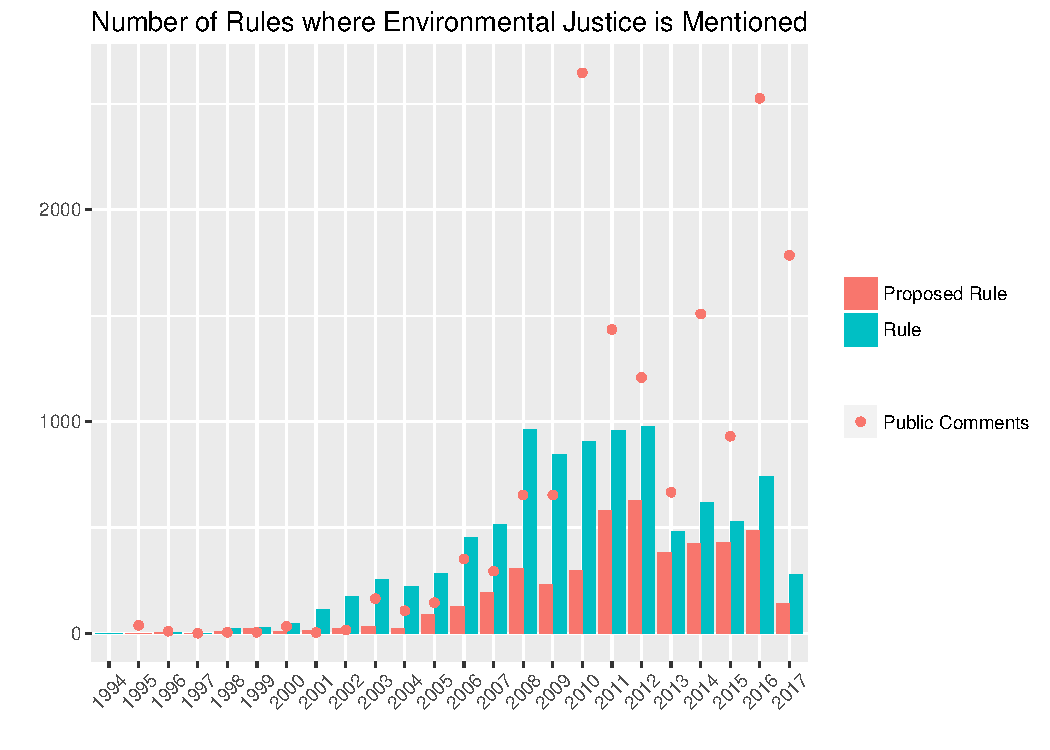
\includegraphics[width = 3.5in]{eandj_hist.pdf}
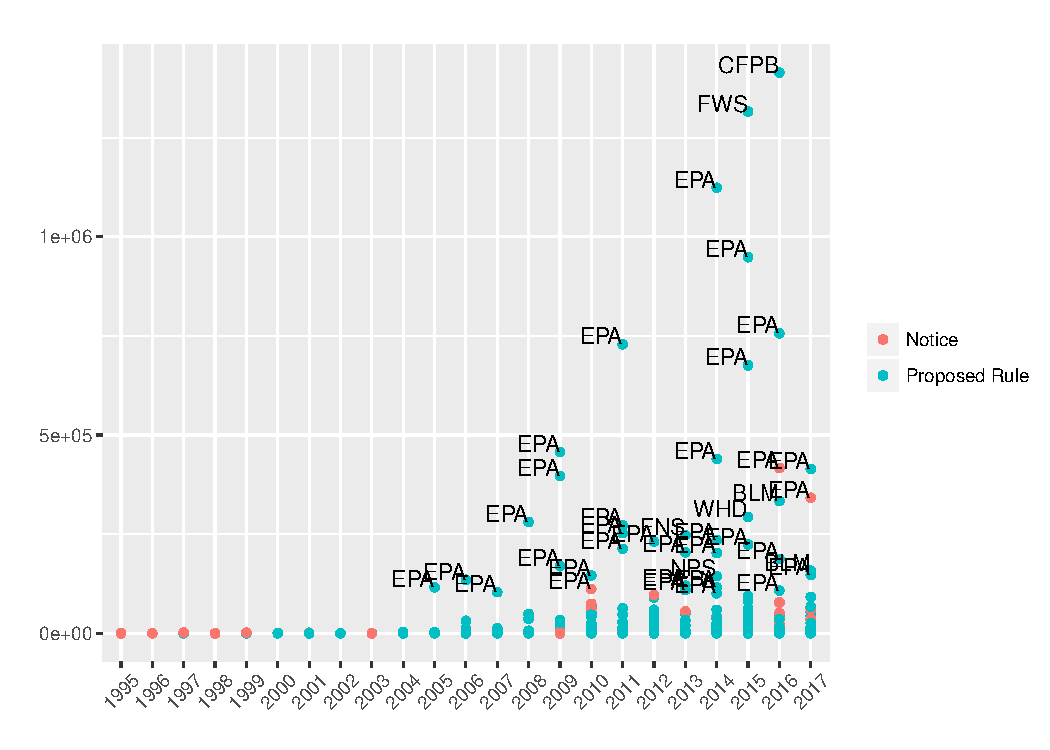
\includegraphics[width =3.5in]{eandj_comments.pdf}
\label{fig:ej}
\end{figure}

Figure \ref{fig:ej} shows that the number of rules and comments increasing over time. This may reflect increased salience of this concept, but it may primarily be the result of the increasing prevalence of searchable texts.  Similarly, the increased number of rules where comments mention environmental justice may reflect growth in the movement but also may reflect more overall comments as technology has made commenting easier. Testing the hypotheses that comments raising environmental justice concerns are related to specific rules where environmental justice is addressed in the final but not in the draft requires rule-specific analysis. 

What we can say from Figure  \ref{fig:ej}  is that each year, more final rules directly address environmental justice when their draft did not. Additionally, there are many rules where environmental justice is mentioned in the public comments and not in the draft. Recently, there are also many rules where environmental justice is raised in the comments but does not make it into the final draft.\footnote{Note that, because not all comments are searchable, this is an underestimate of the number of comments mentioning environmental justice, so we cannot conclude that before 2010, rules were mentioning environmental justice when the comments had not. Additionally, this does not include comments like those of the Bishops who raise justice issues but do not use the phrase ``environmental justice.''} 

% \subsection{Next Steps}
%With these data in hand, the next step is to match each draft and final rule to identify how each changed and to match each comment to its rule to see if the observed changes were suggested in comments. 

\subsubsection{Second-order Representation} Before analysis of whether comments matter, I briefly describe who these commenters are. This is what \citet{Seifter2016Second-OrderLaw} calls ``second-order'' representation. It is insufficient to know which groups participate. We also need to know who these groups represent.

I  investigate who is raising environmental justice concerns in two ways. First, I  identify the top organizational commenters such as tribes, businesses, and nonprofits that are using environmental justice language and investigate who these groups represent. Second, for comments where a citizen signed their name, I  compare surnames to their racial and ethnic identity propensities with respect to the U.S. census. Together these two pieces of information allow me to comment on ``second order'' representation, i.e. not just the extent to which public comments relate to government policy, but the extent to which public comments are representative of the public and of the groups they claim to represent. 


\begin{figure}[!h]
\centering
\begin{tabular}{rlll}
  \hline
 & Organization & Comments & Rules \\ 
  \hline
1 & Earthjustice & 1114782 & 28 \\ 
  2 & Natural Resources Defense Council &  340554 &  8 \\ 
  3 & Sierra Club &  349841 &  5 \\ 
  4 & Alliance for Climate Protection &  253867 &  5 \\ 
  5 & WE ACT for Environmental Justice &    2402 &  3 \\ 
  6 & CREDO &  112879 &  2 \\ 
  7 & Union of Concerned Scientists &   43559 &  2 \\ 
  8 & Earthworks &     308 &  2 \\ 
  9 & Communities for a Better Environment &      21 &  2 \\ 
  10 & Southern Company &       8 &  2 \\ 
  11 & Move On &  165948 &  1 \\ 
  12 & Care2 &   70450 &  1 \\ 
  13 & The Pew Charitable Trusts &   63769 &  1 \\ 
  14 & Hudson-Environmental Action &   35000 &  1 \\ 
  15 & Democracy for America &    4426 &  1 \\ 
  \end{tabular}
  \label{fig:orgs}
  \end{figure}

Figure \ref{fig:orgs} shows the top 15 organizational commenters who used the phrase ``environmental justice'' in their comments, including all organizations who did so on more than one rule or mobilized more than 100,000 such comments. The six organizations responsible for mobilizing more than 100,000 comments and several others on the list are national nonprofit advocacy groups.  We Act and Communities for a Better Environment are both more community-based groups focusing primarily on environmental justice issues. Southern Company is the only corporation on the list
 
 The top mobilizer, Earthjustice, is primarily engaged in litigation on behalf environmental causes. Their website boasts 2.2 million supporters,  but it is not clear who they are or if they play any role in the advocacy strategy. A search on the website returns 360 results for "Environmental Justice," with the top results from staff biographies who work on more local or targeted work such as environmental conditions for the incarcerated, but the environmental justice language used on the main page is relatively mild. For example, ``We are fighting for a future where children can breathe clean air, no matter where they live'' \citep{Earthjustice2017OurWork}. The website does contain Spanish language content. 
 
 The Natural Resources Defense Council is similar to Earthjustice--a national nonprofit funded by donations and focused on litigation--but they also lobby. CREDO Action and MoveOn are more generic progressive mobilizers who lack a systematic focus on environmental justice issues, but occasionally leverage their very large membership lists to support campaigns environmental justice campaigns led by others \citep{MoveOn.org2017MoveOn.OrgAction,CREDO2017CREDOTogether}. The Alliance for Climate Protection is a more of an elite political group founded by former Vice President Al Gore. 
 
 We Act and Communities for a Better Environment both have environmental justice in their central mission statement. We Act was founded by community leaders in Harlem, NY, to fight environmental racisms and advocate for better air quality \citep{WEACT2017WEChange}. Communities for a Better Environment has projects throughout California, but seems particularly active in Oakland \citep{CBECAL2017CommunitiesEnvironment}. Much of the content of their website is in both English and Spanish. Both organizations focus primarily on ``low-income communities of color'' and thus frame their work with respect to race and class. While both organizations participated in national policymaking We Act is more focused on communities in Harlem and New York whereas Communities for a Better Environment casts a wider frame: "CBE’s vision of environmental justice is global--that’s why the organization continues to participate in such international efforts as the Indigenous Environmental Network and the Global Week of Action for Climate Justice" \citep{CBECAL2017CommunitiesEnvironment}.
 
 The Southern Company comments are too few to count as mass mobilization. Companies do sometimes fund mobilization campaigns, but all of 8 of these comments were submitted by the Southern Company. Interestingly, the company repeatedly raises research into environmental justice concerns in order to frame these issues as a legitimate but unresolved scientific debate that is not yet conclusive enough to base regulations on: "People with lower SES are exposed to almost an order of magnitude more traffic near their homes (Reynolds et al., 2001), and live closer to large industrial sites and are exposed to more industrial air pollution (Jerrett et al., 2001). Legitimate health concerns must be addressed. But adopting standards with a scientific basis so uncertain that health improvement cannot be assured is not sound public health policy." Like many companies they claim to represent their customers as "electric generating companies and their customers are expected to bear much of the burden" of regulations \citep{Hobson2004CommentCompany}.
 
 With respect to second-order representation, it appears that the groups most often using the language of environmental justice may do so sincerely, but do not themselves represent affected communities. Several groups representing local communities and led by community leaders have participated, but not nearly as often or with the same intensity as the ``big greens.'' Finally, a third class of commenter appears to be raising environmental justice issues as a way to re-frame them as ongoing debates and thus undermine their urgency. In a way, the fact that an energy company felt compelled to acknowledge and question environmental justice concerns suggests their importance for policy outcomes.

Next, I attempt to estimate the racial distribution of those who comment using environmental justice language. This can only be done for individuals who commented separately from mobilizing organizations and signed their full name on their comment. 
Figure \ref{ejcommentsbyrace} shows two ways of estimating the racial distribution of commenters who raise ``environmental justice'' concerns in their comments. Both methods use the reported racial identities associated with surnames as recorded in the 2010 census\footnote{I recode ``Hispanic'' as ``Latinx'' in both cases because the prediction method assumes a forced choice that includes ``Hispanic'' as a primary racial category} and are based on a limited sample of 327 commenters who signed their name with a surname matching census records.  The first is based on the proportion of people with a given surname that identified as belonging to each racial category (from this limited set of options). The estimated proportion of each race for this sample is simply the average of proportions identified with each surname. This is likely the most accurate way to represent the racial distribution of a set of surnames, but it does not assign specific individuals to racial categories. The second method does. It predicts the race of each individual in the sample based on their surname given the distribution of racial categories reported by people with that surname and the proportion of each race in the U.S. population. Thus, while a surname may be more common among people who identify as black rather than as white, there may still be more White people with that surname and this method would predict that the person is White. For this reason, the portion of individuals predicted to be White (right) is higher than in the probabilistic distribution (left). 

\begin{figure}[h!]
\caption{Probabilistic (Left) and Predicted (Right) Race from Census Surnames}
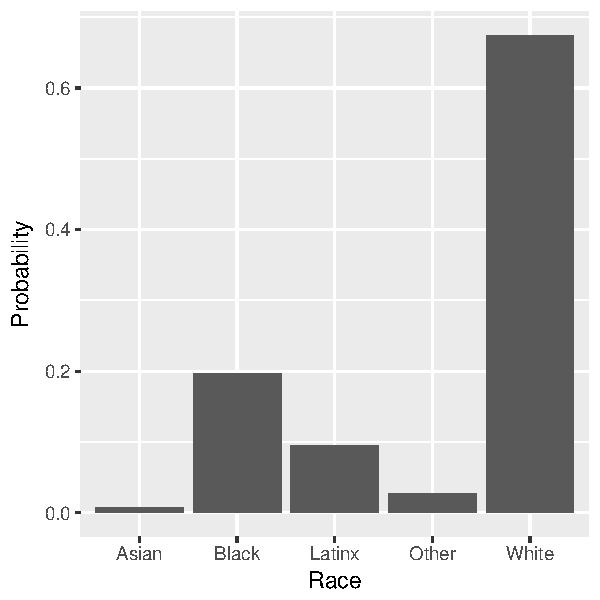
\includegraphics[width = 3in]{race_prob.pdf}
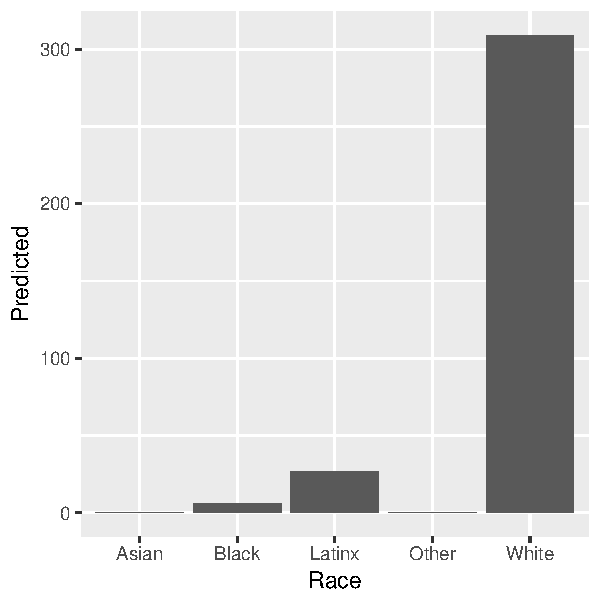
\includegraphics[width = 3in]{race_pred.pdf}
\label{ejcommentsbyrace}

\end{figure}

Compared to estimates from the 2010 census, this sample of commenters is disproportionately Black and less than proportionally Latinx or Asian, with just slightly fewer Whites relative to the national population. 

Figure \ref{ejwordsbyrace} shows the most common words used in comments with respect to the predicted race of each commenter in the sample. As there are very few predicted non-White commenters in the sample, it is unwise to infer too much from this figure. 


\begin{figure}[h!]
\caption{Common Words by Race}
\begin{tabular}{ccc}
White & Latinx & Black\\
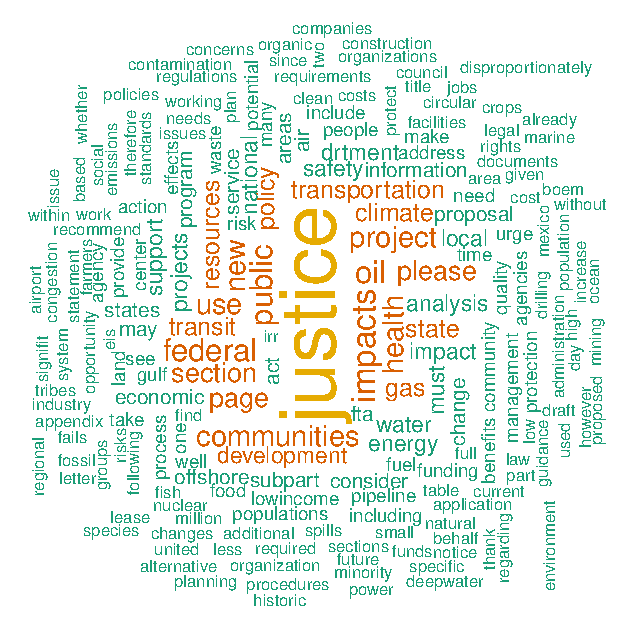
\includegraphics[width = 2in]{ej_white_words.pdf}
&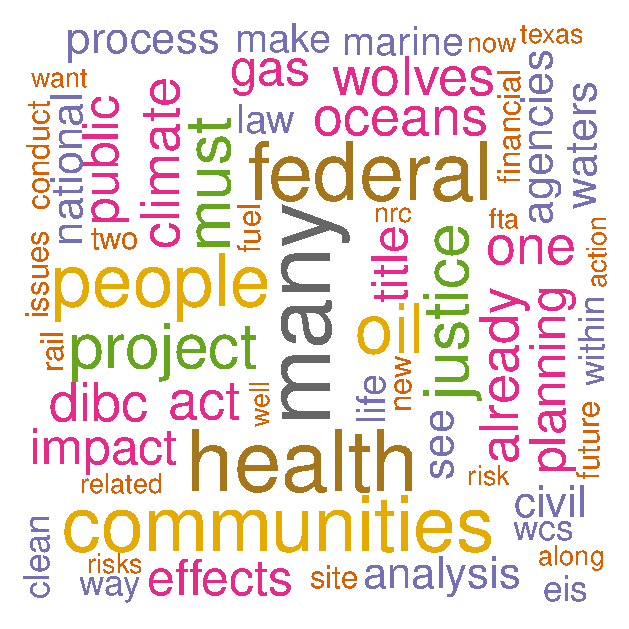
\includegraphics[width = 2in]{ej_latinx_words.pdf}
&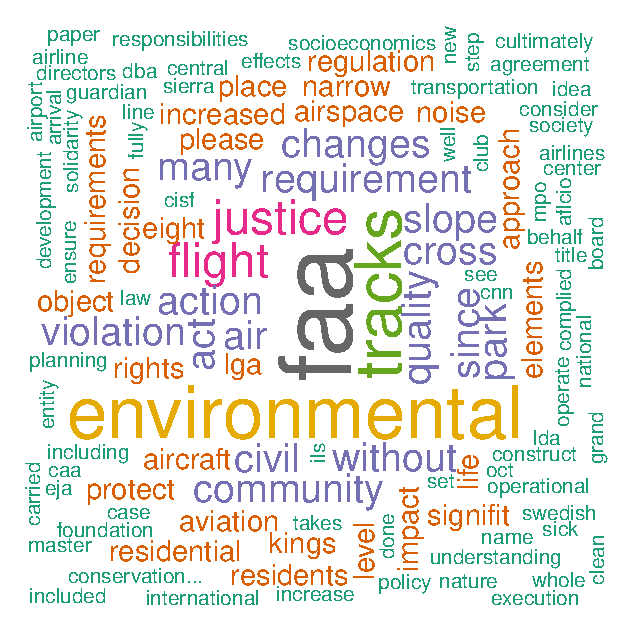
\includegraphics[width = 2in]{ej_black_words.pdf}
\end{tabular}
\label{ejwordsbyrace}
\end{figure}

% Time allowing I will also investigate different pathways to influence such as how rule-specific environmental justice concerns were raised in congressional hearings and reports. 


\subsection{Results: Are final rules more likely to address environmental justice after comments do so?}


This subsection presents results from an analysis of draft rules, comments, and final rules. Descriptively, figure \ref{ejwinrate} shows that in general, most rules that do not address environmental justice in the draft but these issues are raised in the comments, do not end up addressing them in the final version. It appears that it may have been the case in 2006 and 2007 but since then the number of rules receiving comments raising environmental justice concerns has grown while the number of rules that end up adding it has remained the same. Since 2015, there has been a decline in both the number of rules adding environmental justice and the number of rules where commenters demanded it, especially in 2017. One way to interpret figure \ref{ejwinrate} would be to say that commenters saw a potential ally in President Obama and increased their demands for environmental justice, but that these increased demands had little effect. However, a better approach would be to estimate a statistical model of the effect of comments on the change from draft to final rules. This is what I do.


\begin{figure}[h!]
\caption{Rules With Comments Addressing EJ on a Draft That Did Not}
\centering
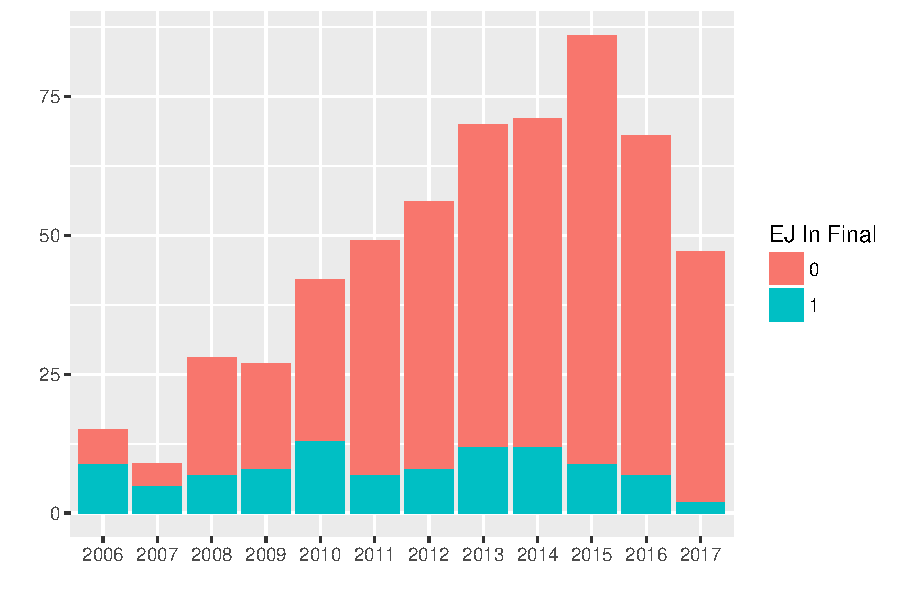
\includegraphics[width = 3.5in]{ej_win_rate.pdf}
\label{ejwinrate}
\end{figure}




I estimate a logit regression where the outcome is whether environmental justice was addressed in the final rule and the predictors are whether it was addressed in the draft rule, whether it was addressed in the comments, and the total number of comments received. 

\begin{align*}
  \hat{EJ in Final} = \Bigg\{ \begin{array}{lll}
    1 & if &  \beta_0 + \beta_1 EJ in Draft + \beta_2 EJ in Comments + \beta_3 Total Comments  + \epsilon > 0\\
0 & otherwise &  
  \end{array}
\end{align*}

As logit coefficients are not easily interpretable, I calculate predicted probabilities for the types of rules of interest, i.e. rules where environmental justice was not raised in the draft, \textit{EJinDraft}=0.  Figure \ref{ejpredicted} shows the predicted probability of a final rule addressing environmental justice when the draft rule did not for all agencies that have ever published a rule addressing environmental justice (left) and the EPA alone (right). The EPA accounts for nearly two-thirds of the cases where environmental justice is raised in the comments on a draft rule that did not address it. We see that the total number of comments has no effect. In contrast, environmental justice being raised in the comments has a statistically significant and substantively large effect. 

Overall the probability across all agencies of adding environmental justice increases from under 2\% to about 9\%. At the EPA, the probability triples from about 6\% to about 18\%. 


\begin{figure}[h!]
\caption{Proposed Rules Not Addressing Environmental Justice (Left: All agencies. Right: Environmental Protection Agency)}
\centering
\noindent
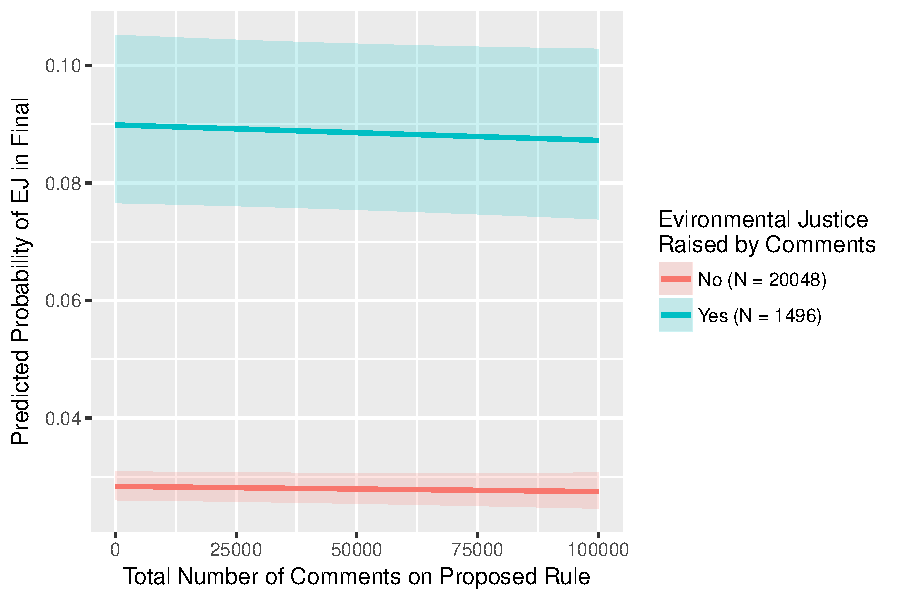
\includegraphics[width = 3.2 in]{ej_prob_env_nprms.pdf}
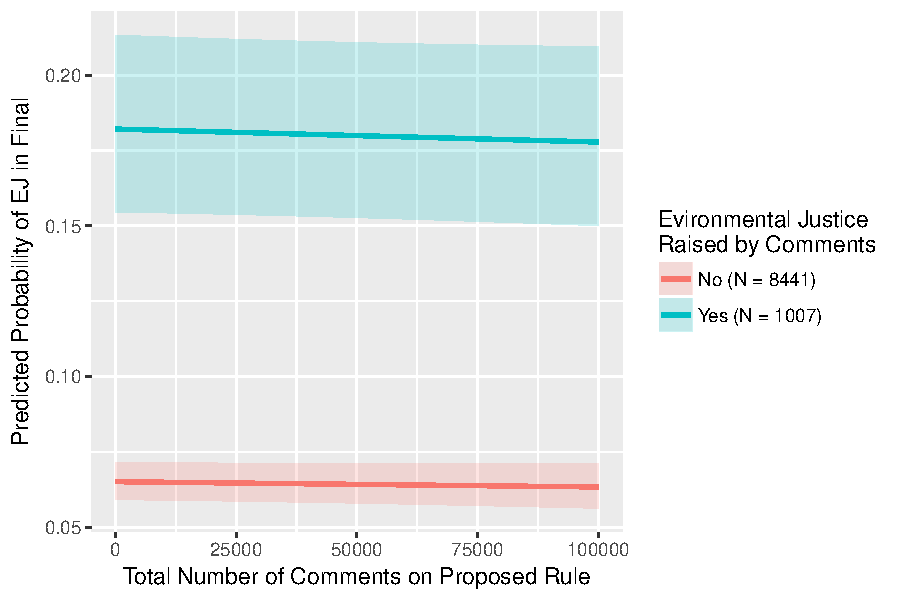
\includegraphics[width = 3.2 in]{ej_prob_epa_nprms.pdf}
\label{ejpredicted}
\end{figure}

To examine the degree to which this result is generalizable, figure \ref{ejlogitagencies} presents predicted probabilities for each agency, showing that the range of predicted probabilities are systematically higher when environmental justice. There is considerable variation among agencies and only a few agencies have statistically significant different estimates, but the agencies where effects are largest and most significant are exactly the agencies we would expect to be influenced by comments raising environmental justice concerns. They are agencies that deal with environmental issues with distributive consequences. 


\begin{figure}[h!]
\caption{Proposed Rules Not Addressing Environmental Justice}
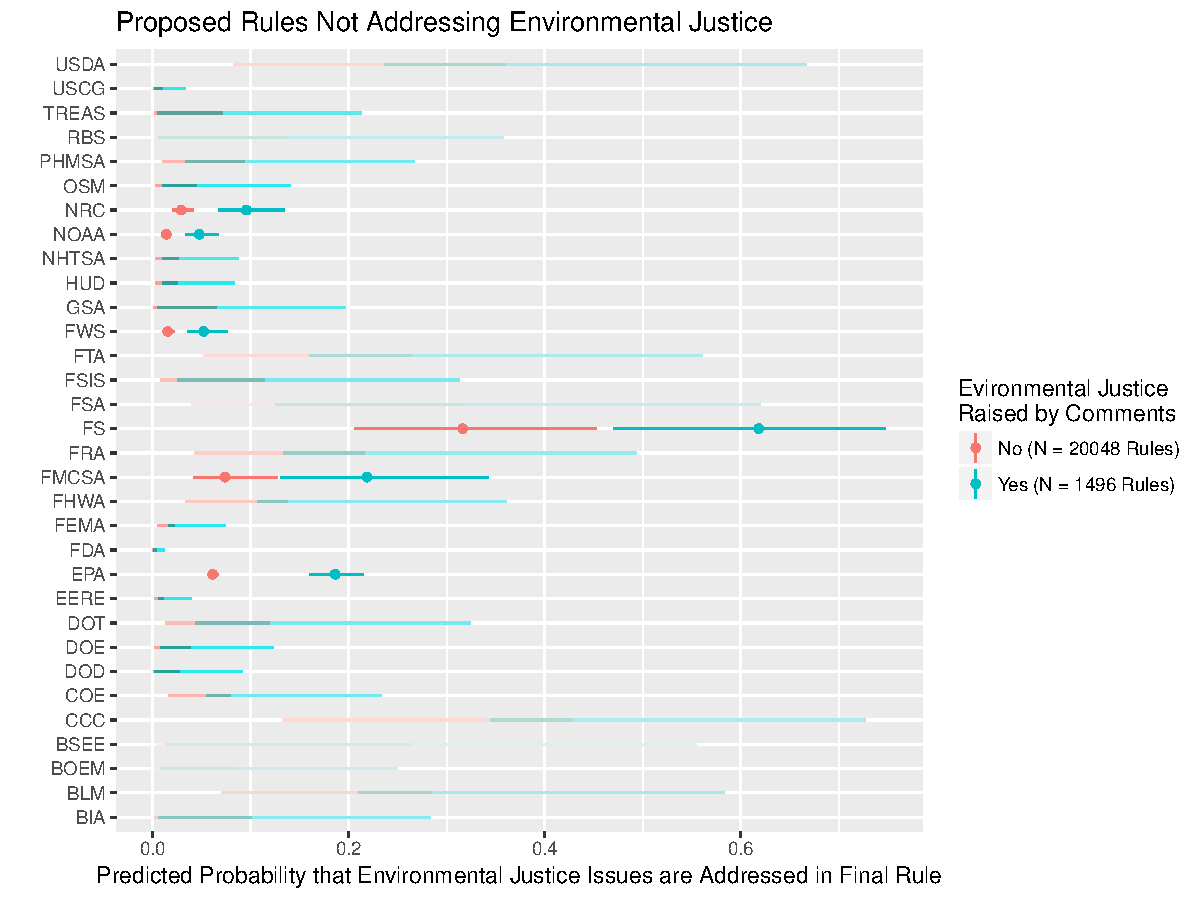
\includegraphics[width = \textwidth]{ej_prprob_by_agency.pdf}
\label{ejlogitagencies}

\end{figure}

As the EPA accounts for the largest portion of the data, we are most confident in this result, but the EPA is not the agency with the largest predicted effects. The Forest Service has a predicted 30\% difference between rules that do and do not receive comments raising environmental justices concerns. This may be because the forest service is mainly in the business of managing forests, leasing timber rights, and controlling wildfires. These types of decisions may have acute distributional effects that may not be the initial focus of the agency. Once raised, however, addressing such effects fits squarely in their mission. Though not statically significant the Department of Agriculture and Bureau of Land Management, who make similar kinds of decisions, also have large predicted probabilities. Similarly, the Federal Railroad Administration, Department of Transportation, Federal Highway Administration, Federal Motor Carrier Safety Administration, and Federal Transportation Administration (which aids local transportation projects) all have large probability distributions. These agencies are making decisions about infrastructure projects with implications for neighborhood environments and air quality. Environmental justice may often come up, but there may be a lot of variation in whether the agency then decides if they are relevant to transportation policies and projects that are primarily about neither environmental nor justice concerns. 

Research agencies, including the National Research Council, National Oceanographic and Atmospheric Administration and Fish and Wildlife Service all had statistically significant but small spreads. In these cases, we can be confident of the correlation, but understand that it is a rare occurrence, which makes sense if most research does not have direct environmental justice consequences, but agencies are open to adding analysis of these issues if when they are raised. 

\section{Conclusion}
This analysis has illustrated the importance of ideas in policymaking and cross-sectional statistical results suggest that rules where issue frame like environmental justice are raised have a higher probability that policymakers consider the effects on marginalized populations. Importantly this relationship seems to be conditional on an institutional environment that is predisposed to such an analysis. Furthermore, it is important to note that the policy outcomes suggested by environmental justice analysis depend on how minority populations are defined. In some cases, those raising environmental justice concerns present it as an issue of wealth or income inequality, leading policy to account for disparate impacts on low-income populations. In other cases, groups raise claims rooted in cultural practices, such as fish consumption among certain tribes. As occurred in the Mercury Rule, analysis in subsequent drafts of the policy used evaluative criteria specific to these communities. 

The ability of a frame like environmental justice to construct certain populations as deserving of consideration means that policy outcomes will depend on the specific environmental justice concerns raised. In this respect, second-order representation may become important. National  advocacy organizations may frequently request that regulators protect ``all people'' or even ``low-income communities of color.'' However, this more generic advocacy may not lead to the same outcomes as groups that present specific local environmental justice grievances that are unique to a community. In between generic progressive advocacy organizations and community-based organizations are organizations like Earthjustice who, despite their national focus, frequently engaged in community-specific litigation and thus raise these local concerns in national policymaking. 

In the end, the above analysis offers some clarity on a poorly understood but important mechanism of American policymaking. It offers some hope that citizen opinions may be heard through direct democracy institutions built into bureaucratic policymaking.  The examination of second-order participation validates some of the skepticism about who participates. It is elite groups who participate, even with respect to an issue like environmental justice. However, government responsiveness does not seem to depend on mass mobilization or elite support. Compared to cases where environmental justice issues were not raised, when they are, we see a significantly higher probability that they will be addressed by policymakers. 

% \section{Conclusion}

% 
\includegraphics[height = .5cm]{spam}

\theendnotes

\footnotesize
\bibliographystyle{apsr.bst} 
\bibliography{Mendeley.bib}

\end{document}
